% *** Authors should verify (and, if needed, correct) their LaTeX system  ***
% *** with the testflow diagnostic prior to trusting their LaTeX platform ***
% *** with production work. IEEE's font choices can trigger bugs that do  ***
% *** not appear when using other class files.                            ***
% The testflow support page is at:
% http://www.michaelshell.org/tex/testflow/

\documentclass[conference]{IEEEtran}

\usepackage{balance}
\usepackage{url}
%\usepackage{breakurl}
%\usepackage[breaklinks]{hyperref}
\usepackage{graphicx}
% correct bad hyphenation here
\hyphenation{op-tical net-works semi-conduc-tor}



\begin{document}
\title{Spreadsheets are Code \large{\\An Overview of Software Engineering Approaches applied to Spreadsheets}}


\author{\IEEEauthorblockN{Felienne Hermans, Bas Jansen, Sohon Roy, Efthimia Aivaloglou, Alaaeddin Swidan and David Hoepelman}
\IEEEauthorblockA{\{f.f.j.hermans, b.jansen, s.roy-1, e.aivaloglou, alaaeddin.swidan\}@tudelft.nl, d.j.hoepelman@student.tudelft.nl}
\IEEEauthorblockA{Delft University of Technology}
\IEEEauthorblockA{The Netherlands}
}


\maketitle

\begin{abstract}
Spreadsheets can be considered to be the world's most successful end-user programming language. In fact, one could say spreadsheets \emph{are} programming. This paper starts with a comparison of spreadsheets to software: spreadsheets are similar in terms of applications domains, expressive power and maintainability problems. We then reflect upon what makes spreadsheets successful: liveness, directness and an easy deployment environment seem contribute largely to their success.

Being a programming language, several techniques from software engineering can be applied to spreadsheets. We present an overview of such research directions, including spreadsheet testing, reverse engineering, smell detection, clone detection and refactoring. Finally, open challenges and future plans for the domain of spreadsheet software engineering are presented.
\end{abstract}

\IEEEpeerreviewmaketitle

\section{Introduction}
In addition to professional programmers who are employed to build, maintain and test software, there is also a large body of people programming not as a job, but as as a means to an end. These workers, often called \emph {end-user programmers} write queries, small scripts or spreadsheets to support their daily jobs. The number of end-user programmers in the USA alone is conservatively estimated at 11 million compared to only 2.75 million other, professional programmers~\cite{Scaf2005}. Among end-user programmers, especially the use of spreadsheets is popular. These are used for a large variety of different tasks, from scheduling to financial reporting and from investment analysis to corporate budgeting in all sorts of domains, from small shops to multinationals. 

Especially in the financial domain, spreadsheets are ubiquitous. In 2004, the International Data Corporation interviewed 118 business leaders and found that 85\% were using spreadsheets in financial reporting and forecasting~\cite{Panko2008}.  Financial intelligence firm CODA reported in 2008 that 95\% of all U.S. companies use spreadsheets for financial reporting~\cite{Panko2008}. In a survey held in 2003 by the US Bureau of Labor Statistics~\cite{BLS2003}, over 60\% of 77 million surveyed workers in the US reported using spreadsheets, making this the third most common use of computers, after email and word processing. A more recent survey among 95 companies world-wide, placed spreadsheets fourth, after email, browsing and word processing, accounting for 7.4\% of computer time~\cite{Wellnomics2007}. The Dutch Bureau of Statistics investigates computer literacy among Dutch civilians every year, and has reported a rise in people able to use formulas in spreadsheets from 44\% in 2006 to 54\% in 2013~\cite{CBS2013}.

As artifacts of end-user programming, spreadsheets often play a role similar to source code in many companies: they support important organizational processes and often business decisions are taken based on the information calculated and presented in spreadsheets~\cite{hermans_supporting_2011}.

While spreadsheets are commonly used, their users often have little training as programmers. In spite of that, they often face many of the challenges of professional developers, like choosing which functions to use~\cite{Ko2004}, or understanding someone else's code~\cite{Ko2011}. Since spreadsheets, like software, frequently contain errors~\cite{Panko1998}, end-users test, verify and debug their programs~\cite{Hermans2013-Cascon,Ko2004-Why}.

These issues that end-users face---issues of program construction, maintenance, testing and debugging---have been topics of research in the programming and software engineering community for decades. Given the similarities between spreadsheets and source code, it is feasible to transform software engineering methods, tools and techniques to make them applicable to spreadsheets. This exactly has been the approach of a number of researchers over the last decade. This paper highlights their past achievements, challenges and future research directions. 

\section{End-user programming}
End-user programming has been a topic of study for decades, mainly started by Nardi~\cite{Nardi1993} in her investigations into spreadsheet use in office workplaces. According to Nardi, the difference between an end-user programmer and a professional programmer lies in their goals. It is the responsibility of a professional developer to build, debug, maintain and sometimes test software for others to use, while end-user developers create programs to support their own domain of expertise, like teaching, planning or bookkeeping~\cite{Ko2011}. As such, programs that end-users create are, by definition, not meant for others to use, while professional programming has the goal of producing code for others to use. 

One of the core problematic aspects of end-user programming is that sometimes the created artifacts evolve from personal solutions to programs used by many colleagues. When that happens, an end-user suddenly, often unintended and unprepared, has to take on challenges of professional developers, like testing, maintaining and generalizing their creations. 

%\bas{And furthermore also when they use the spreadsheets for themselves, the software engineeering like problems do not go away. A spreadsheet for personal use suffers from the same problems that can have significant impact.}

\section{Spreadsheets are Code}
While end-user programming takes on many forms, and their users can be as diverse as system administrators~\cite{Barrett2004} or interaction designers~\cite{Ko2004, myers_how_2008}, spreadsheets can be considered to be the most successful form of end-user programming.

 % Ko also names: natural scientists [Carver et al. 2007; Segal 2007], software architects [Lakshminarayanan et al. 2006], bioinformatics professionals [Letondal 2006], web designers [Rode and Rosson 2003]

Spreadsheets are crucial tools for many workers, enabling millions of users to do reporting, planning, scheduling and all else needed to succeed in their jobs. Of course, not all spreadsheets are full-fledged applications: some are simply used for word processing with an easier layout and do not even contain formulas. Spreadsheets however are also commonly used to create applications, or to perform business critical calculations. We argue this second group of spreadsheets can and should be seen as source code, paving the way to apply methods from software engineering to them. 

In the following paragraphs, we outline three reasons why spreadsheets systems are programming languages, and spreadsheets are code.

\subsection{Similar Goals}
Firstly, spreadsheets are used for very similar problems, like financial calculations or data manipulation. In such situations, spreadsheets play a role that can also be played by software. 

In many cases, the end-users have investigated alternatives, for example, the use of 'off the shelf' solutions for their data or analysis needs. However, these are often expensive and do not fit their needs exactly. A second alternative could be custom made software, either by software engineers within the company or by a contractor. These projects unfortunately have the tendency to go over budget and sometimes have disappointing results. Weighting all options: expensive off the shelf product, unsatisfying tailor made software, making a spreadsheet themselves often seems a non-expensive and simple solution for many end-users.

\subsection{Similar Expressive Power}

\begin{figure}
  \begin{center}
  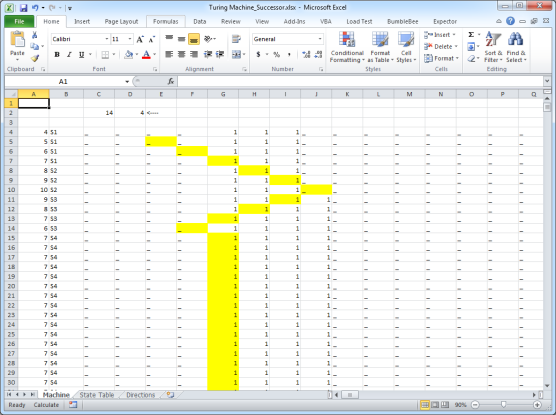
\includegraphics[width=\columnwidth]{fig/turing.png}
  \caption{A Turing machine implementation in Excel, using only formulas. Rows represents consecutive states of the machine and the cells in yellow indicate its head.}
  \label{fig:visical}
  \end{center}
\end{figure} 

Secondly, spreadsheets have quite some expressive power. In fact, spreadsheet formulas are Turing complete, even without taking Visual Basic for Applications code into account. Using formulas only, you can construct a Turing machine, see Figure \ref{fig:visical}~\cite{Turing2013}. Without using VBA it is not possible to continuously update cells, so moving the head is mimicked by using one row in the spreadsheet to represent one state of the tape. Each following line represents the state of the tape after one transition, and the head of the machine is visualized with conditional formatting.

\subsection{Similar Maintainability Issues}

Finally spreadsheets suffer from typical software problems, including, but not limited to the issues below.

\textbf{Long life span} In some cases, spreadsheets are specifically created for one time use, but more often they stay `alive': enhanced with more data, reused for next year's budget or modified for a different department. Our research shows that spreadsheets have an average lifespan of five years~\cite{hermans_supporting_2011}.

\textbf{Many different users} During this long lifespan, spreadsheets are frequently shared among coworkers. On average, twelve different people work with one spreadsheet, performing a variety of tasks on them, including data entry, error checking and analysis~\cite{hermans_supporting_2011}.

\textbf{Lack of documentation} We found that only one in three spreadsheets contain documentation, where we considered even a basic manual as documentation, we did not limit the definition to real technical documentation with design decisions. And still, two thirds of spreadsheets did not contain any explanation~\cite{hermans_supporting_2011}.

\textbf{Quality issues} Finally, like software, there have been many accounts of big impact errors involving spreadsheets. From somewhat silly errors, like an overbooked Olympic stadium~\cite{Kelso2012}, to career wrecking data analysis mistakes~\cite{Herndon2014}, the stories of errors are numerous. The European Risk Interest Group keeps a list of these ‘spreadsheet horror stories’ on their website\footnote{\url{www.eusprig.org/horror-stories}}.

\section{Reflections on Spreadsheet Success factors}
Given the wide adoption of spreadsheets, one could wonder why spreadsheets are as successful as they are. In this section we list three reasons contributing to their success.

\subsection{Live Programming}

\begin{figure}
  \begin{center}
  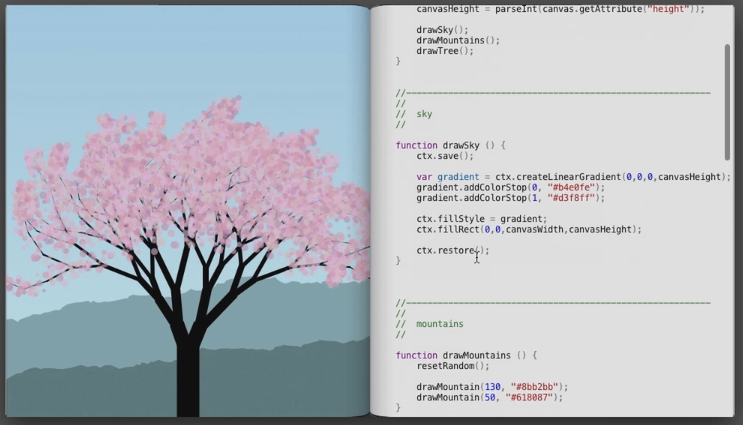
\includegraphics[width=\columnwidth]{fig/bret.png}
  \caption{Live programming: on the right the source code and on the left its instantiation of the code which changes immediately when the code is updated, screenshot from ~\cite{Victor2012}.}
  \label{fig:bret}
  \end{center}
\end{figure} 

First proposed as a design principle by Maloney and Smith ~\cite{maloney_directness_1995} liveness indicates that a user interface is always active and reactive. According to \cite{maloney_directness_1995} in a live interface \emph{``objects respond to user actions, animations run, layout happens, and information displays are updated continuously''}. More recently  live programming has found its way to the public eye, among others by Bret Victor in his talk `Inventing on Principle'~\cite{Victor2012}. Figure \ref{fig:bret}, taken from Victor's talk, illustrates the idea of live programming: on the right, we have source code and on the left, we have the result of that code, in this case: a tree. Modifying the code will immediately affect the tree.
 
This liveness is also present in spreadsheet systems. When a users enters a formula and presses enter, the see the result, without any effort such as compilation. Liveness of spreadsheets powers their flexibility, often praised as their key success factor.

\subsection{Directness}
Another benefit of spreadsheets is that their interface combines data, metadata and calculations together in one view, and provides the user with easy access to all. Just by clicking a formula, one can manipulate it. This is often called `directness': \emph{``the feeling
that one is directly manipulating the object''}~\cite{shneiderman_direct_1983}. From a cognitive perspective, directness in computing means \emph{``a small distance between a goal and the actions required of the user to achieve the goal''} ~\cite{burnett_visual_2001}.

Maloney and Smith describe directness as the fact that a user can  \emph{``can initiate the process of examining or changing the attributes, structure, and behavior of user interface components by pointing at their graphical representations directly, as opposed to navigating through an alternate representation.''}~\cite{maloney_directness_1995}

This is how a spreadsheet works too. Instead of navigating to a code behind, a class or an object, spreadsheet user have all ingredients (data, metadata and calculations) in one view, and can access them with one view. 

We have often wondered why more advanced spreadsheet users did not use a database or source code, which would have enforced a more structured approach. In our experience, spreadsheet users felt that the distance between the meta-data---designing the tables---, the data---filling them---and the analysis----queries---was too big, posing a cognitive load too high.

 %This is not that surprising, understanding dependencies of code is one of the challenges that developers still face, even advanced IDE's like Eclipse or Visual Studio do not solve this entirely. \todo{ref for this}

\subsection{One-click deployment}
Another problem that end-user programmers in a company setting face is the problem of deployment. Some more advanced users write, for example, Python scripts to analyze data, but are then left with the question of how to get that to run on your neighbor's workstation, with a slightly different version of the operating system, a newer Office and different language settings? Spreadsheets are so universal that almost everyone has a spreadsheet program on their machine. With that, a spreadsheet becomes an executable package with data and calculations packed together, that can run anywhere.

\section{Achievements}
As said, a core approach of research into end-user programming has been to transfer methods from software engineering to end-user languages, and this has been eagerly applied spreadsheet research. This section presents an overview of successful research directions following this strategy.

\subsection{Testing}
One of the programming concepts that found its way to spreadsheets the earliest is testing, with `What You See Is What You Test' (WYSIWYT) by Rothermel \emph{et al.}~\cite{Rothermel1997}. In this paradigm, spreadsheet users have to mark formula outcomes are correct or incorrect, after which the WYSIWYT system calculates which formulas led to the checked values and increases their testedness. 

An evaluation of WYSIWYT showed that their approach had an average fault detection percentage of 81\% which is \emph{``comparable to those achieved by analogous techniques for testing imperative programs."}~\cite{Rothermel2000}. Other studies have confirmed the applicability of testing to spreadsheets~\cite{Kruck2006}. Related is the elegant work of Burnett on spreadsheet assertions that allows spreadsheet users to define assertions and propagates them through the cell dependencies using a similar propagation system \cite{Burnett2003}.

An downside of the WYSIWYT approach is that it requires an annotation of right and wrong values as input, meaning extra effort for the user. When inspecting spreadsheets from practice, we noticed that spreadsheet users often already add simple tests to their spreadsheets expressed with formulas. An example of such a spreadsheet is shown in Figure \ref{fig:test-example}. In the EUSES corpus~\cite{fisher_euses_2005}, 9.8\% of formulas are such test formulas, which we deemed common enough to be exploited. Hence, we built a tool called Expector that can detect these formulas, store them in a test suite and subsequently calculate coverage and run the tests~\cite{Hermans2013-Cascon}.

\begin{figure}
  \begin{center}
  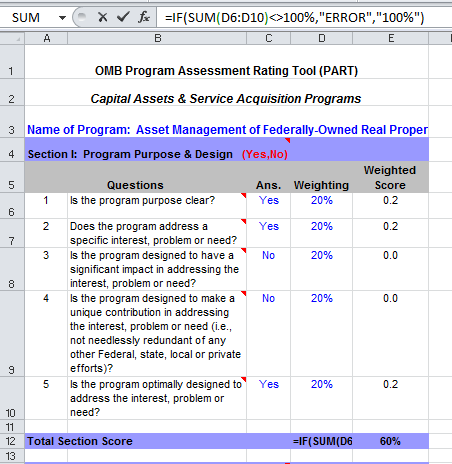
\includegraphics[width=5cm]{fig/test-example.png}
  \caption{A spreadsheet with a test formula in cell D12 expressing that the SUM of the values in D6:D10 should be equal to 100\%}
  \label{fig:test-example}
  \end{center}
\end{figure} 


\subsection{Reverse Engineering} 
Like software, spreadsheets often suffer from a lack of documentation. In a field study we found, only one in three spreadsheets contained documentation~\cite{hermans_supporting_2011}. Despite this lack of documentation, users do are often have to understand spreadsheets created by someone else~\cite{Ko2011,hermans_supporting_2011}. An approach that was therefore explored by several researchers is to reverse engineer existing spreadsheets in some way.

\subsubsection{Extracting class diagrams}
There have been a number of approaches to extract class diagrams from spreadsheets. We described a method to do so by observing that spreadsheets typically contain three types of data: actual data organized in groups, computations over these groups, and dependencies between them, closely resembling object oriented systems with classes, methods and dependencies~\cite{hermans_automatically_2010}. based on this observation, we implemented a method to transform spreadsheets to class diagrams and evaluated it on the EUSES corpus~\cite{fisher_euses_2005}. We found that we were able to extract diagrams similar to a manually created benchmark in 40\% of spreadsheets.

Following this work, Cunha \emph{et al.}~\cite{cunha_automatically_2010} described an approach to infer ClassSheets models~\cite{engels_classsheets:_2005} from spreadsheets, by detecting and exploiting functional dependencies. Their method was validated in a method similar to ours. They manually extracted tables from 27 spreadsheet examples taken from \cite{management_2003}. They found that their method was able to detect correct ClassSheets in about 70\% of the cases.

Specifically focusing on the spreadsheets made by scientists, de Vos \emph{et al.}~\cite{vos_g.:_2012} have designed a methodology to extract ontologies in the form of class diagrams from spreadsheets. While their described method is currently manual, they state it could be automated too. 

%(maybe include) Isakowitz et al. proposed a related methodology to infer a logical layer of existing spreadsheets [10], but their process in not completely automatic, it requires human intervention in some cases.

\subsubsection{Dataflow visualization}
In addition to approaches to extract data models as documentation from spreadsheets, there have also been a number of approaches aimed at extracting and visualizing dependencies between cells. One could say that spreadsheets consist of two layers: \emph{visual}: the way in which cells are organized into rows, columns, data blocks and worksheets, and \emph{dependency}: the way in which cells refer to each other.

\begin{figure}
	\centering
	\setlength{\fboxsep}{0pt}
	\setlength{\fboxrule}{1pt}
	\fbox{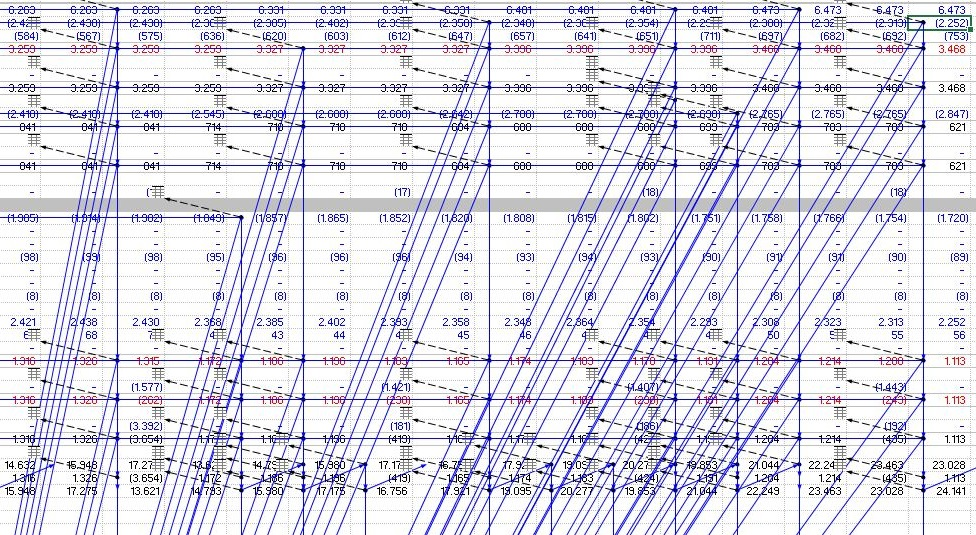
\includegraphics[width=\linewidth]{fig/ComplexDependence}}
	\caption{Spreadsheet shown in Microsoft Excel with the `trace dependents' option enabled. As can be seen in this picture, this feature does not always support easy understanding.}
	\label{fig:ComplexDependence}
\end{figure}

Firstly, Excel itself contains a feature to overlay a spreadsheet with a dependency graph, which, unfortunately becomes incomprehensible for large and complex spreadsheets, as shown in Fig \ref{fig:ComplexDependence}. Observing that this feature did not always support spreadsheet users, we studied needs that industrial spreadsheet users have when working with spreadsheets~\cite{hermans_supporting_2011}. The results confirmed that that most important information needs of spreadsheet users concern the structure of formula dependencies. To meet this demand we developed an approach for the automatic generation of \emph{leveled} data-flow diagrams from spreadsheets. The diagrams are organized in levels and are thus able to represent larger spreadsheets without becoming cluttered, as shown in Figure \ref{fig:worksheet-view}. We implemented the approach and evaluated it with a group of 27 users at Robeco, a Dutch financial services company. The results indicated that end-users consider the tool helpful; the visualizations help them to create story lines for explaining spreadsheets to colleagues, and they scale well to large and complex spreadsheets. 

\begin{figure}
  \begin{center}
  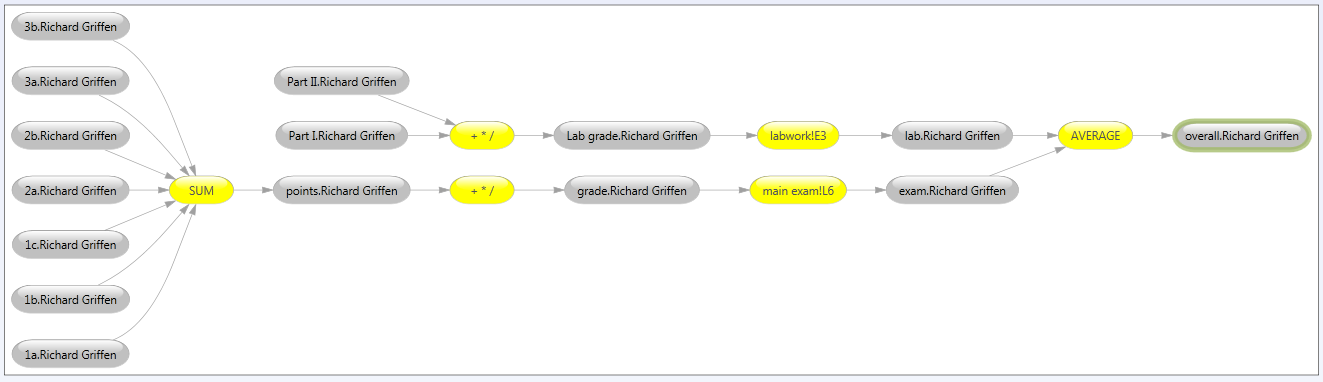
\includegraphics[width=\columnwidth]{fig/formula-view.png}
  \caption{Formula view of the Leveled Dataflow Visualization as presented in \cite{hermans_supporting_2011}}
  \label{fig:formula-view}
  \end{center}
\end{figure} 

\begin{figure}
  \begin{center}
  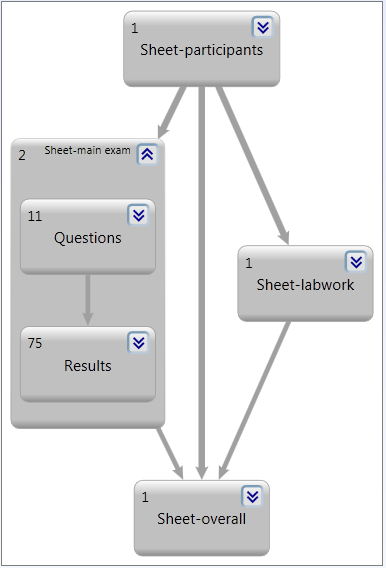
\includegraphics[width=5cm]{fig/worksheet-view.png}
  \caption{Worksheet view of the Leveled Dataflow Visualization as presented in \cite{hermans_supporting_2011}}
  \label{fig:worksheet-view}
  \end{center}
\end{figure} 

There have been several related efforts to support spreadsheet users in comprehension. Igarashi \emph{et al.} developed a fluid visualization technique based on overlaid animation for better understanding of spreadsheets \cite{igarashi1998fluid}. Shiozawa \textit{et al.} proposed a technique of cell dependence visualization in 3D based on an interactive lifting up operation \cite{shiozawa19993d}. Ballinger \textit{et al.} developed a visualization toolkit that could ease understanding of spreadsheets through visual abstractions in the form of images that emphasize on layout and dependency rather than values of cells \cite{ballinger2003spreadsheet}. The toolkit was successfully tested on a corpus of 259 spreadsheets but there was no information about the source or size of the spreadsheets. 

In addition to these generic works on dataflow visualization, there is also work specifically tailored towards the spreadsheets used by scientists~\cite{de_vos_methodology_2015}. In this paper de Vos \emph{et al.} propose a semi automatic method to infer the calculation workflow underlying a set of spreadsheets. The starting point of our methodology is, like in our approach, the cell dependency graph. The difference is that 1) De Vos \emph{et al.} automatically aggregate all cells in the graph that represent instances and duplicates of the same quantities, based on analysis of the formula syntax. The method also needs an ontology of the spreadsheets domain as input, which is then used to prune the data flow graph by selecting only relevant nodes. They have performed three case studies showing that their generated calculation models approximate the ground truth calculation workflows, both in terms of content and size, but are not a perfect match.

\subsection{Smell Detection} 
While the work on reverse engineering certainly proves useful when users want to understand or migrate their spreadsheets, sometimes users still got lost in unnecessarily complex formulas. This, again, resembled the problems in course code. Therefore we have coined the idea of \emph{spreadsheet smells}, taking the code smells metaphor of Fowler as source of inspiration~\cite{Fowl1999}.

\subsubsection{Formula-level Smell Detection}
We started by defining smells within individual formulas and we found that many smells defined for code also applied nicely to spreadsheets~\cite{hermans_detecting_2014}. As an example, consider conditional complexity. Most spreadsheet systems contain IF and other conditional formulas, so spreadsheet formulas too can suffer from conditional complexity, when many conditionals are nested within one formula. An example of a formula suffering from the \emph{conditional complexity} smell is shown in Figure \ref{fig:ConditionalComplexity}.

\begin{figure}
  \begin{center}
  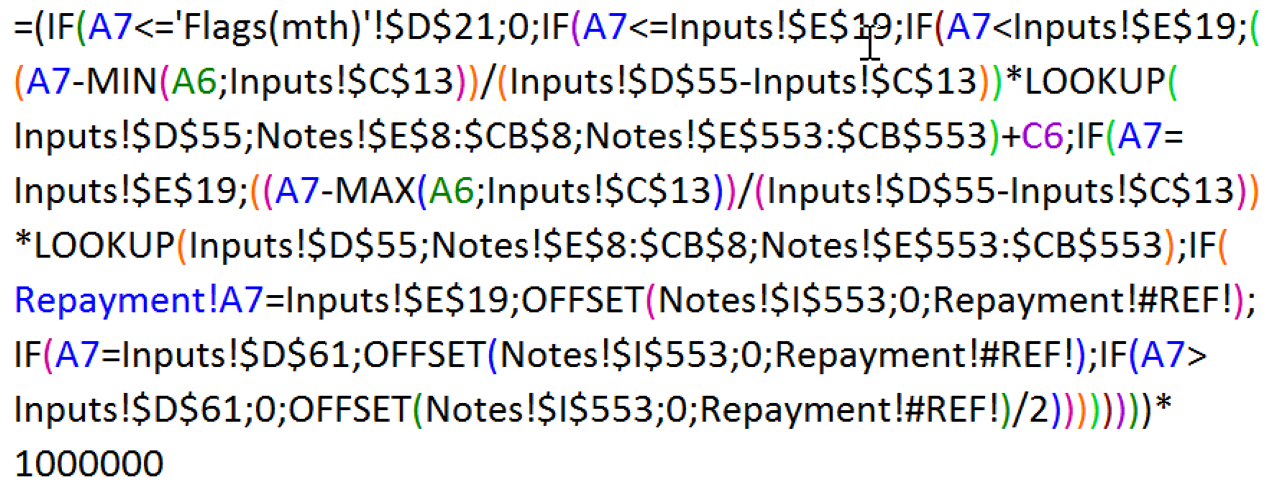
\includegraphics[width=\columnwidth]{fig/ConditionalComplexity.png}
  \caption{Formula suffering from the Conditional Complexity smell, inhibiting easy readability}
  \label{fig:ConditionalComplexity}
  \end{center}
\end{figure} 

Other code smells need small modifications to be applicable to spreadsheets: the \emph{many parameters} smell becomes \emph{many references}: a formula that references a long list of different ranges in a spreadsheet is as smelly as a method with lots of parameters, and the \emph{long method} smell becomes \emph{multiple operations}: a formula that uses a large number of different functions can be hard to understand. 

After defining the smells for spreadsheets, we performed an empirical evaluation in which we found that smells occurred within 42.7\% percent of spreadsheets in the EUSES corpus~\cite{fisher_euses_2005} and that \emph{Multiple References} is the most common. We also evaluated the smells with 10 spreadsheets and their users in practice, and found two actual faults with the \emph{duplication}. Also, spreadsheet users agreed that the
smells revealed which the formulas were least maintainable.

More recently, we compared two datasets: one containing spreadsheets which users found unmaintainable, and a version of the same spreadsheets rebuilt by professional spreadsheet developers. The results show that the improved versions suffered from smells to a lesser degree, increasing our confidence that presence of smells indeed coincides with users finding spreadsheets hard to maintain~\cite{Jansen2015}.

%\subsubsection{Spectrum-Based Smell Detection}
%\todo{SBFL}

\subsubsection{Data Smell Detection}
Cunha \emph{et al.} studied smells in spreadsheets too, however they focus on smells in the data, such as cells that do not follow a normal distribution or have a big string distance to other cells in the same region, and thus might be typos. They analyzed 180 spreadsheets from the EUSES corpus, in which they found 3,841 cells suffering from their smells. By manual inspection of the cells, they confirmed that more than 20\% of the detected smelly cells point to a possible problem in the spreadsheet~\cite{cunha_towards_2012}.

Related work into smells in data was done by Barowy \emph{et al.} who present a tool called CheckCell that identifies cells that have an unusually high impact on the spreadsheet's computations. In an evaluation, the authors showed that CheckCell outperforms standard outlier detection techniques. It successfully finds injected typographical errors produced by a generative model trained with data entry from 169,112 Mechanical Turk tasks~\cite{barowy_checkcell:_2014}.


\subsubsection{Structural Smell detection}
In addition to smells occurring within data or within a single formula, smells can occur in the organization of the spreadsheet, for example is a formula refers to a large number of cells in another worksheet. This is comparable to Fowler's \emph{Feature Envy} smell, where a method of class A uses a large number of fields from class B, and hence can be considered `envious' of the class B.

We defined three more structural smells in addition to \emph{Feature Envy}, namely: \emph{Inappropriate Intimacy}, \emph{Middle Man} and \emph{Shotgun Surgery}~\cite{hermans_detecting_2012-1}. We again performed a quantitative and qualitative evaluation of our approach, where we first investigated the occurrence of inter-worksheet smells in the EUSES~\cite{fisher_euses_2005} corpus and found that 23.3\% of spreadsheets suffered from at least on of the smells, with \emph{Feature Envy} being the most common smell. We also conducted a series of ten case studies at the above described company Robeco. In these case studies we found that inter-worksheet smells can indeed reveal weaknesses in spreadsheets and that subjects confirmed their negative impact on maintenance.

\subsection{Clone detection}
Like in source code, clones or `copy-pasting' occurs in spreadsheets too, although there are important differences. 
Copy-pasting in spreadsheets is common: spreadsheet users typically mimic abstraction by copying a similar formula down or left over multiple rows or columns. An example of this is given in the lower part of Figure \ref{fig:ambig}, where the formulas in cells D2 and F2 are copied down and the formula in B2 is copied left.

\begin{figure}
  \begin{center}
  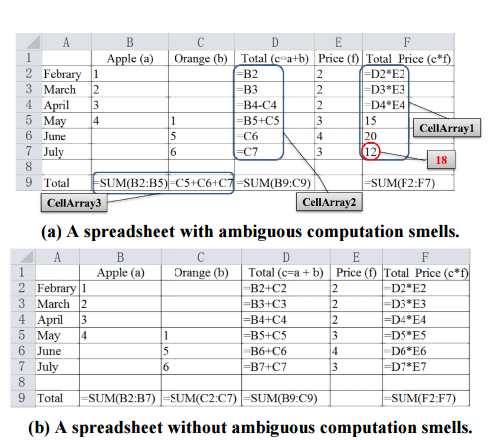
\includegraphics[width=\columnwidth]{fig/ambig.png}
  \caption{Two versions of a spreadsheet, with and without ambiguous computation. Taken from \cite{dou_is_2014}}
  \label{fig:ambig}
  \end{center}
\end{figure} 

However, some forms of copying are error prone. In our research we have focused on \emph{data clones}: copies made with the `paste as values' option supported by Excel.  We designed a detection algorithm~\cite{hermans_data_2013} to help spreadsheet users in finding and refactoring clones, based on existing clone detection algorithms working on source code~\cite{DBLP:conf/cascon/Johnson93}. In addition to exact clones, our approach also detects \emph{near-miss clones}, those where minor to extensive modifications have been made to the copied fragments~\cite{DBLP:conf/icsm/Roy09}. Our approach was  validated both quantitatively and qualitatively. Firstly, we analyzed the EUSES corpus~\cite{fisher_euses_2005} to calculate the precision and performance of our algorithm and to understand how often clones occur. Secondly, we performed two case studies: one with a large budget spreadsheet from our own university and a second one for a large Dutch non-profit organization, for which we analyzed 31 business critical spreadsheets.

Dou \emph{et al.} studied clones in spreadsheets too, focusing on the degeneration of clones formulas ~\cite{dou_is_2014}. They state that spreadsheet formulas are initially often similar in a row or column. When a spreadsheet evolves however, some cells in such a group will be updated, due to ad hoc modifications or undisciplined copy-and-pastes. Dou \emph{et al.} state these cells suffer from the ambiguous computation smell. They find that such smells are common and likely harmful and propose a tool called AmCheck which automatically detects and repairs ambiguous computation smells. They present a case study on the spreadsheets of the EUSES corpus~\cite{fisher_euses_2005}, showing that 44.7\% of the spreadsheets with suffer from at  least  one  kind  of ambiguous computation smell. They then randomly selected 700 sampled smelly groups of cells and manually confirmed that 319 (45.6\%) of them were true smelly cell arrays. 

\subsection{Refactoring}
A final direction on which end-user research has focused on---a logical step after research on smells---is refactoring of end-users artifacts. 

We defined a refactorings corresponding to our smells~\cite{hermans_detecting_2014} and applied them to 10 spreadsheets we received from employees at Robeco, demonstrating that a combination of one or more refactorings from our set could relieve smells in 87\% of smelly formulas. 

Inspired by our work on spreadsheet smells, Badame and Dig~\cite{badame_refactoring_2012} developed a tool called RefBook that supported a number of refactorings for spreadsheet formulas including extract column, replace awkward formula, string to dropdown, introduce cell name, and extract literal. While some of their refactorings can relieve known code smells---for example extract column makes formulas shorter, thus addressing the \emph{multiple operations} smell---their refactorings were not directly related to smells. RefBook was evaluated on 28 users in an online experiment showing that RefBook increases spreadsheet programmer
productivity, increases the reliability of transformations, and increases the quality of spreadsheets. Furthermore they studied the EUSES corpus to show that their refactorings can be widely applied. For example, 27\% of formulas demonstrated some form of duplication, meaning that Extract Column could be applied to simplify the spreadsheet.

After this, we combined the above two approaches in a new spreadsheet refactoring tool called Bumblebee, which allows a formula to be transformed into another by defining a transformation rule. Therefore, BumbleBee is more generic than RefBook, which only supported a fix number of refactorings~\cite{hermans_bumblebee:_2014}. However, initially, this approach has the downside that it can only consider one formula, and not the spreadsheet as a whole, meaning some of RefBook's refactorings like Extract Formula and Introduce Cell Name were not supported. This was addressed by the work of Hoepelman~\cite{hoepelman_thesis_2015}, which furthermore introduced new refactorings including Inline Formula and Introduce Conditional Aggregate.

\subsection{Conclusion}
To summarize, we conclude that a diverse range of approaches aimed at source code are applicable to end-user programming in general and spreadsheets in particular. From testing to smells, and from refactoring to reverse engineering, software engineering methods and techniques transfer well and, a broad range of evaluations demonstrate that end-users benefit them.

%This all has to do with understanding and improving quality we still want to support understanding domain/calculation.Our work and that of others was all 100\% automated, what we have learned, if we want to continue with reverse engineering, we need more support from the user, both the creator and human level intelligence (a generic user): we both want to do large studies with generic users like the labeling game and make support for users to add more (domain) knowledge to the sheets.

\section{Challenges} 
Now that we have described the key successes in the application of software engineering to spreadsheets, including testing, reverse engineering, smell detection, clone detection and refactoring, we direct our attention to challenges in researching software engineering methods in spreadsheets. 

\subsection{End-user's Perception and Self Perception}
One of the core challenges of performing research on end-user programming in general, is that users do not see themselves as programmers. In one case where we were working with an investment banker, who was almost insulted when we, impressed with a risk management dashboard he built with Excel, called him a programmer. Because end-user programmers do not self-identify as developers, they often are unaware of tools, methods and techniques that could support them in their programming efforts.

The perception of end-user programmers as not being `real' programmers is not limited to how programmers view themselves, but also to how they are seen by others. Coworkers, especially those themselves trained as professional developers, often fail to recognize and sometimes even belittle their programming efforts, while professional developers in the workplace could offer great support and could ease technology transfer of spreadsheet solutions.

\subsection{Lack of Best Practices}
A challenge that follows from the previous one is the lack of standards. Since spreadsheets and their creators are not seen as source code and programmers respectively, they are often outside of the scope of a diverse range of professionalization efforts within companies. Software, but also numerous processes are standardized; spreadsheets on the other hand are rarely. While a number of spreadsheet standards exist\footnote{\url{http://www.fast-standard.org/}},\footnote{\url{http://www.ssrb.org/standards}},\footnote{\url{http://www.spreadsheetsafe.com/}}, these have to date not found widespread adoption. 

This lack of standards means spreadsheets can be created in many different ways, which inhibits easy comprehension and maintenance, but also makes it harder to automatically analyze and process spreadsheets.

\subsection{Lack of Data}
Spreadsheets often contain models and calculations of vital importance to companies, and therefore their users are reluctant to share them with researchers. This is a big challenge with industrial research in general, and spreadsheets in specific. Contrary to source code, which developers often share on online platforms like GitHub, spreadsheet users typically do not share theirs. 

While there are a number of public datasets available~\cite{fisher_euses_2005, Hermans2015, conf/msr/BarikLSSM15}, only one of these (\cite{Hermans2015}) stems from a company. And even then, we lack information about their creation and the maintenance process around them. Process information that is often available for source code repositories, like issues and version control history, are missing from spreadsheets, prohibiting us from deeply understanding the problems with spreadsheets. We have worked together with companies providing us with data~\cite{hermans_supporting_2011, hermans_detecting_2012, hermans_detecting_2012-1, hermans_detecting_2014, Jansen2015} enabling us to study spreadsheets \emph{in the wild}, however unfortunately, that came at the price of reduced repeatability, as we were not allowed to share these spreadsheets.

\subsection{Performance of research tools}

While many spreadsheets are relatively small, spreadsheets can also grow extremely large over their long lifespan. The biggest spreadsheet from the Enron set had no less than 175 worksheets, and about 10\% of spreadsheets in the corpus have 10 or more worksheets. Large spreadsheets, especially those with heavy connections between the worksheets are hard for users to understand and maintain, but also seem to hinder adoption of research tools, especially for those aimed at supporting maintenance and comprehension. For example, the above Igarashi \emph{et al.} reported that their animations degrade for spreadsheets larger than 400 cells~\cite{igarashi1998fluid} Compared to spreadsheets that are found in the industry, 400 cells is a very low limit. We ourselves have also found that parsing and analyzing large numbers of formulas can be more time-consuming that one would expect. Thus it appears that although these tools typically perform well on laboratory examples, industrial adoption is far away for real-life spreadsheets, as tools get unreasonably slow on large spreadsheets.

%For useful visualization we have to leave the cell level, want to look at the computation level (slicing)

\subsection{Proprietary Software} 
A final challenge that we identify in working with spreadsheets is the fact that the most common spreadsheet system, Microsoft Excel, is proprietary and closed source. This sometimes makes analysis hard, especially in regards to parsing spreadsheet formulas, which is needed for research efforts, including testing and refactoring approaches. While a formal specification is available, this specification consist of about 30 pages worth of production rules, making it a demanding effort to reimplement. This resulted in the fact that many researchers has to reverse engineer and approximate the excel formula grammar.  Various papers have attempted to cover a small subset. For example, in his thesis, Badame presents a grammar that is clearly not covering all possible formulas~\cite{badame_thesis_2012}. Other papers process formulas, but do not share their parser or grammar, like the CheckCell paper~\cite{barowy_checkcell:_2014} and the works by Cunha \emph{et. al.}\cite{cunha_automatically_2010, cunha_towards_2012}. We recently released a version of the grammar as an open source project, capable of parsing 99.9\% of formulas in the EUSES and Enron dataset~\cite{Aivaloglou_2015}.

Another problem is that Excel limits the power of add-ins, most notably by disallowing access to the undo-stack, but also limiting the possibilities to traverse cell dependencies deeper than one level. These both increased our difficulties in developing the refactoring plugin~\cite{hermans_bumblebee:_2014}.

Obviously, one could avoid such these issues by implementing a whole spreadsheet system for scratch, but there is a trade off between easy extendability and power of tools on the one hand and realism on the other hand. As a researcher you also want to attract a large group of people to be able to try your tools, so there is something to say for building on top of Excel, even in the presence of the above challenges.

%an approach that has been followed by \todo{Forms/3}. Sestoft also developed his own spreadsheet system, but not as a means for plugins or add-ons necessarily, but more to explore what it entails. 

\section{Future opportunities}
In the previous sections we have described a number directions in which the application of software engineering to spreadsheets  has proven to be successful. Given these achievements and the challenges we identified in terms of perception of end-users, best practices, lack of data, size and performance of spreadsheets, we identify the following viable directions for future work in the area of spreadsheet software engineering.

%\subsection{Continuation of the refactoring and testing work}
%In contrast to the work on smells that have been tried in practice and spurred numerous follow up works and has been picked up by a larger research community, refactorings and testing need to be made more applicable.

\subsection{Performance}
Understandability and maintainability are not the only issues with large spreadsheets, large spreadsheets can also suffer from serious performance problems. 

Some researchers have attempted to improve spreadsheet performance in various ways, for example, Pichitlamken \emph{et a.l}~\cite{7_pichitlamken_kajkamhaeng_uthayopas_kaewpuang_2010} proposed a method to offload a simulation model built in spreadsheets into a grid of computing resources. Their tool, while useful, was developed for a very specific set of conditions, making it difficult to apply to spreadsheets in general. A related effort is the work by Abramson \emph{et al.} in \cite{6_abramson_roe_kotler_mather_2001} who presented ActiveSheets, a solution designed to evaluate ``otherwise sequential'' custom functions of Excel spreadsheets, by creating a middle layer that processes the requests for evaluations. Finally, there is ExcelGrid \cite{10_nadiminti_chiu_teoh_luther_venugopal_buyya_2004}, in which a middle ware tool was designed and built connecting an Excel spreadsheet with either a private or a public cluster. 

The fact that there is some preliminary research done in this direction, indicates that this is a problem worthy of more research. But, while the above tools and techniques do improve performance in the spreadsheets under study, they do not take the content of the spreadsheet into account, by for example identifying hotspots in the spreadsheets calculation. We believe that by combining High Performance Computing with smell detection and refactoring, tailored spreadsheet improvements could be made.

\subsection{Deeply Understanding Spreadsheets in the Enterprise}
So far, research on spreadsheets, both ours and that of other research groups, have focused on individual spreadsheets and their users. In reality, spreadsheets are often part of a larger end-user ecosystem, where users, for example, import data from a data warehouse, process it in a spreadsheet and then write a report about it in Word. We see the broadening of the scope of end-user programming as a very viable direction for future research. 

This research direction will aim to understand why people continue to resort to `home brew' solutions while there are software systems in place. What functionality or power do they miss in existing tools? Understanding what drives people to spreadsheets will support us in building supporting or replacing tools.

\subsection{Domain-Specific Spreadsheets}
Not all spreadsheets are created equally. While working with spreadsheets in practice we have seen that there are several high-level classifications to be made. For example: some spreadsheets are used for financial modeling and project future revenues and costs along a time-axis, other spreadsheets are used for a calculation on a single point in time, for example cost price calculations. In other cases spreadsheets are used purely for reporting purposes and are lacking any complex calculations. In some spreadsheets the calculations are even missing, the spreadsheet is just a collections of lists and is actually used as a database. We hypothesize that each of those categories of spreadsheets needs a different type of support. For example, a there might be budget specific smells or tests, which only help users when they are making a budget, but would would not support a cost price calculations. By analyzing different types of spreadsheets, we could tailor our methods to specialized spreadsheet types.

\subsection{Higher Level of Abstraction}
In previous work we have tried to understand what causes spreadsheets to be error prone. Contrary to our initial hypotheses, studies have found that the level of complexity and coupling in spreadsheets is not that large~\cite{Jansen2015}. So one could wonder what it is that makes spreadsheets error-prone and hard to understand. One hypothesis is that the interface of spreadsheets, with all its freedom for users in how to layout spreadsheets, is a double-edged sword. While allowing the users this total freedom, the interface is not supporting users in making the right choices. One solution we envision is a higher level language to create spreadsheets, as illustrated by Figure \ref{fig:visualLanguage}. When we have a definition of the spreadsheet at a higher level of abstraction, we can subsequently help users to select the right formatting and also support them in changing the layout of the spreadsheet later in the process. 

\begin{figure}
  \begin{center}
  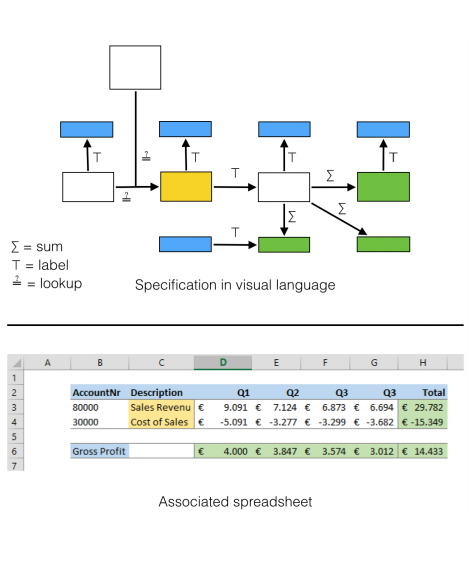
\includegraphics[width=\columnwidth]{fig/visualLanguage.png}
  \caption{We envision the visual language to look like this. On top there is the model the user would create and on the bottom we find the associated spreadsheet}
  \label{fig:visualLanguage}
  \end{center}
\end{figure} 


\subsection{Beyond Formulas}
Spreadsheets themselves are changing, and many vendors, including Microsoft, are trying to enable spreadsheet developers to build more powerful programs. A few initiatives in this direction are QlikView, Tableau and PowerBI. Currently, these tools are certainly bringing more power to end-users, but tool creators are mainly concerned with supporting users to build new analyses and not with helping users maintaining them. We thus hypothesis that that this new generation of end-user programming artifacts will again have unexpectedly long life spans and will also start to suffer from end-user programming smells, and will thus be be in need of testing and refactoring.

\balance

\section{Conclusion}
This paper presents an overview of research papers that apply software engineering to spreadsheets. We first make the case that spreadsheets are code: they are used for similar problems, have similar expressive power and suffer from similar problems. We then reflect upon the success of spreadsheets, what makes them the world's most used programming language for end-users? We assert their liveness, directness and easy deployment are factors contributing to their widespread adoption. 

Because of their similarity to source code, applying methods from software engineering to them has proven a successful research direction for many. In this paper we summarize achievements in the area of testing, reverse engineering, smell detection, clone detection and refactoring. We also highlight challenges in researching spreadsheets, including the perception that spreadsheet developers are not real programmers, the lack of best practices, the lack of readily available data, the difficulties of analyzing large spreadsheets and issues building upon on proprietary software like Excel.

We end this paper by identifying a number of viable research directions, including investigating how to improve the performance of spreadsheets, understanding the process around them, making research more domain specific, raising the level of abstraction for spreadsheet users and finally analyzing reporting artifacts other than spreadsheets.

\balance



% trigger a \newpage just before the given reference
% number - used to balance the columns on the last page
% adjust value as needed - may need to be readjusted if
% the document is modified later
%\IEEEtriggeratref{8}
% The "triggered" command can be changed if desired:
%\IEEEtriggercmd{\enlargethispage{-5in}}


\bibliographystyle{IEEEtran}
% argument is your BibTeX string definitions and bibliography database(s)
\bibliography{references}


% that's all folks
\end{document}


